\begin{figure}[!htb]
	\centering

	\begin{tikzpicture}

		\onslide<1->{
			\node (Before) at (0,0) {
				\begin{tikzpicture}[scale=0.15]
					\coordinate (1) at (-5,-8);
					\coordinate (2) at (10,2);
					\coordinate (3) at (10,10);
					\coordinate (4) at (-7,1);
					\coordinate (5) at (-1,8);
					\coordinate (6) at (-4,-9);
					\coordinate (7) at (5,-3);
					\coordinate (8) at (6,4);
					\coordinate (9) at (3,-5);
					\coordinate (10) at (0,1);

					\draw[thick, blue] (2) -- (10);
					\draw[thick, blue] (1) -- (4);
					\draw[thick, blue] (4) -- (5);

					\foreach \i in {1, ..., 10}{
							\filldraw[black] (\i) circle (4pt);
						}
				\end{tikzpicture}
			};
		}

		\node (Delaunay) at (6,0) {
			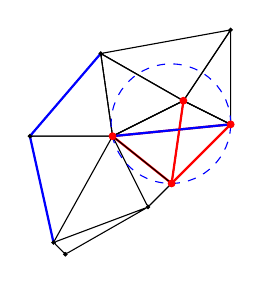
\begin{tikzpicture}[scale=0.15]
				\coordinate (1) at (-5,-8);
				\coordinate (2) at (10,2);
				\coordinate (3) at (10,10);
				\coordinate (4) at (-7,1);
				\coordinate (5) at (-1,8);
				\coordinate (6) at (-4,-9);
				\coordinate (7) at (5,-3);
				\coordinate (8) at (6,4);
				\coordinate (9) at (3,-5);
				\coordinate (10) at (0,1);
				\coordinate (O) at (4.94,2.06);

				\onslide<2->{
					\draw[rounded corners=1pt] (4) -- (5) -- (10) -- cycle;
					\draw[rounded corners=1pt] (1) -- (6) -- (9) -- cycle;
					\draw[rounded corners=1pt] (5) -- (8) -- (10) -- cycle;
					\draw[rounded corners=1pt] (7) -- (9) -- (10) -- cycle;
					\draw[rounded corners=1pt] (3) -- (5) -- (8) -- cycle;
					\draw[rounded corners=1pt] (2) -- (3) -- (8) -- cycle;
					\draw[rounded corners=1pt] (1) -- (4) -- (10) -- cycle;
				}
				\onslide<2, 4, 5>{\draw[rounded corners=1pt] (2) -- (8) -- (10) -- cycle;}
				\onslide<3>{\draw[rounded corners=1pt] (2) -- (7) -- (8) -- cycle;}
				\onslide<2, 5>{\draw[rounded corners=1pt] (2) -- (7) -- (10) -- cycle;}
				\onslide<4>{\draw[thick, red, rounded corners=1pt] (2) -- (7) -- (10) -- cycle;}
				\onslide<3>{\draw[rounded corners=1pt] (7) -- (8) -- (10) -- cycle;}

				\onslide<2, 5>{\draw[thick, blue] (2) -- (10);}
				\onslide<3>{\draw[thick, red] (7) -- (8);}
				\onslide<3>{\draw[dashed, blue] (2) -- (10);}
				\onslide<2->{
					\draw[thick, blue] (1) -- (4);
					\draw[thick, blue] (4) -- (5);

					\foreach \i in {1, ..., 10}{
							\filldraw[black] (\i) circle (4pt);
						}
				}
				\onslide<4>{
					\draw[dashed, blue] (O) circle[radius=5.06];
					\filldraw[red] (2) circle (8pt);
					\filldraw[red] (7) circle (8pt);
					\filldraw[red] (8) circle (8pt);
					\filldraw[red] (10) circle (8pt);

				}
			\end{tikzpicture}
		};

		% % Arrow between them
		\onslide<2->{
			\draw[->, thick] (Before.east) -- (Delaunay.west);
		}

	\end{tikzpicture}

	\caption{Edge constraints for Delaunay triangulation}\label{fig:constrainedDelaunay}
\end{figure}

